\section{Assigment 3}

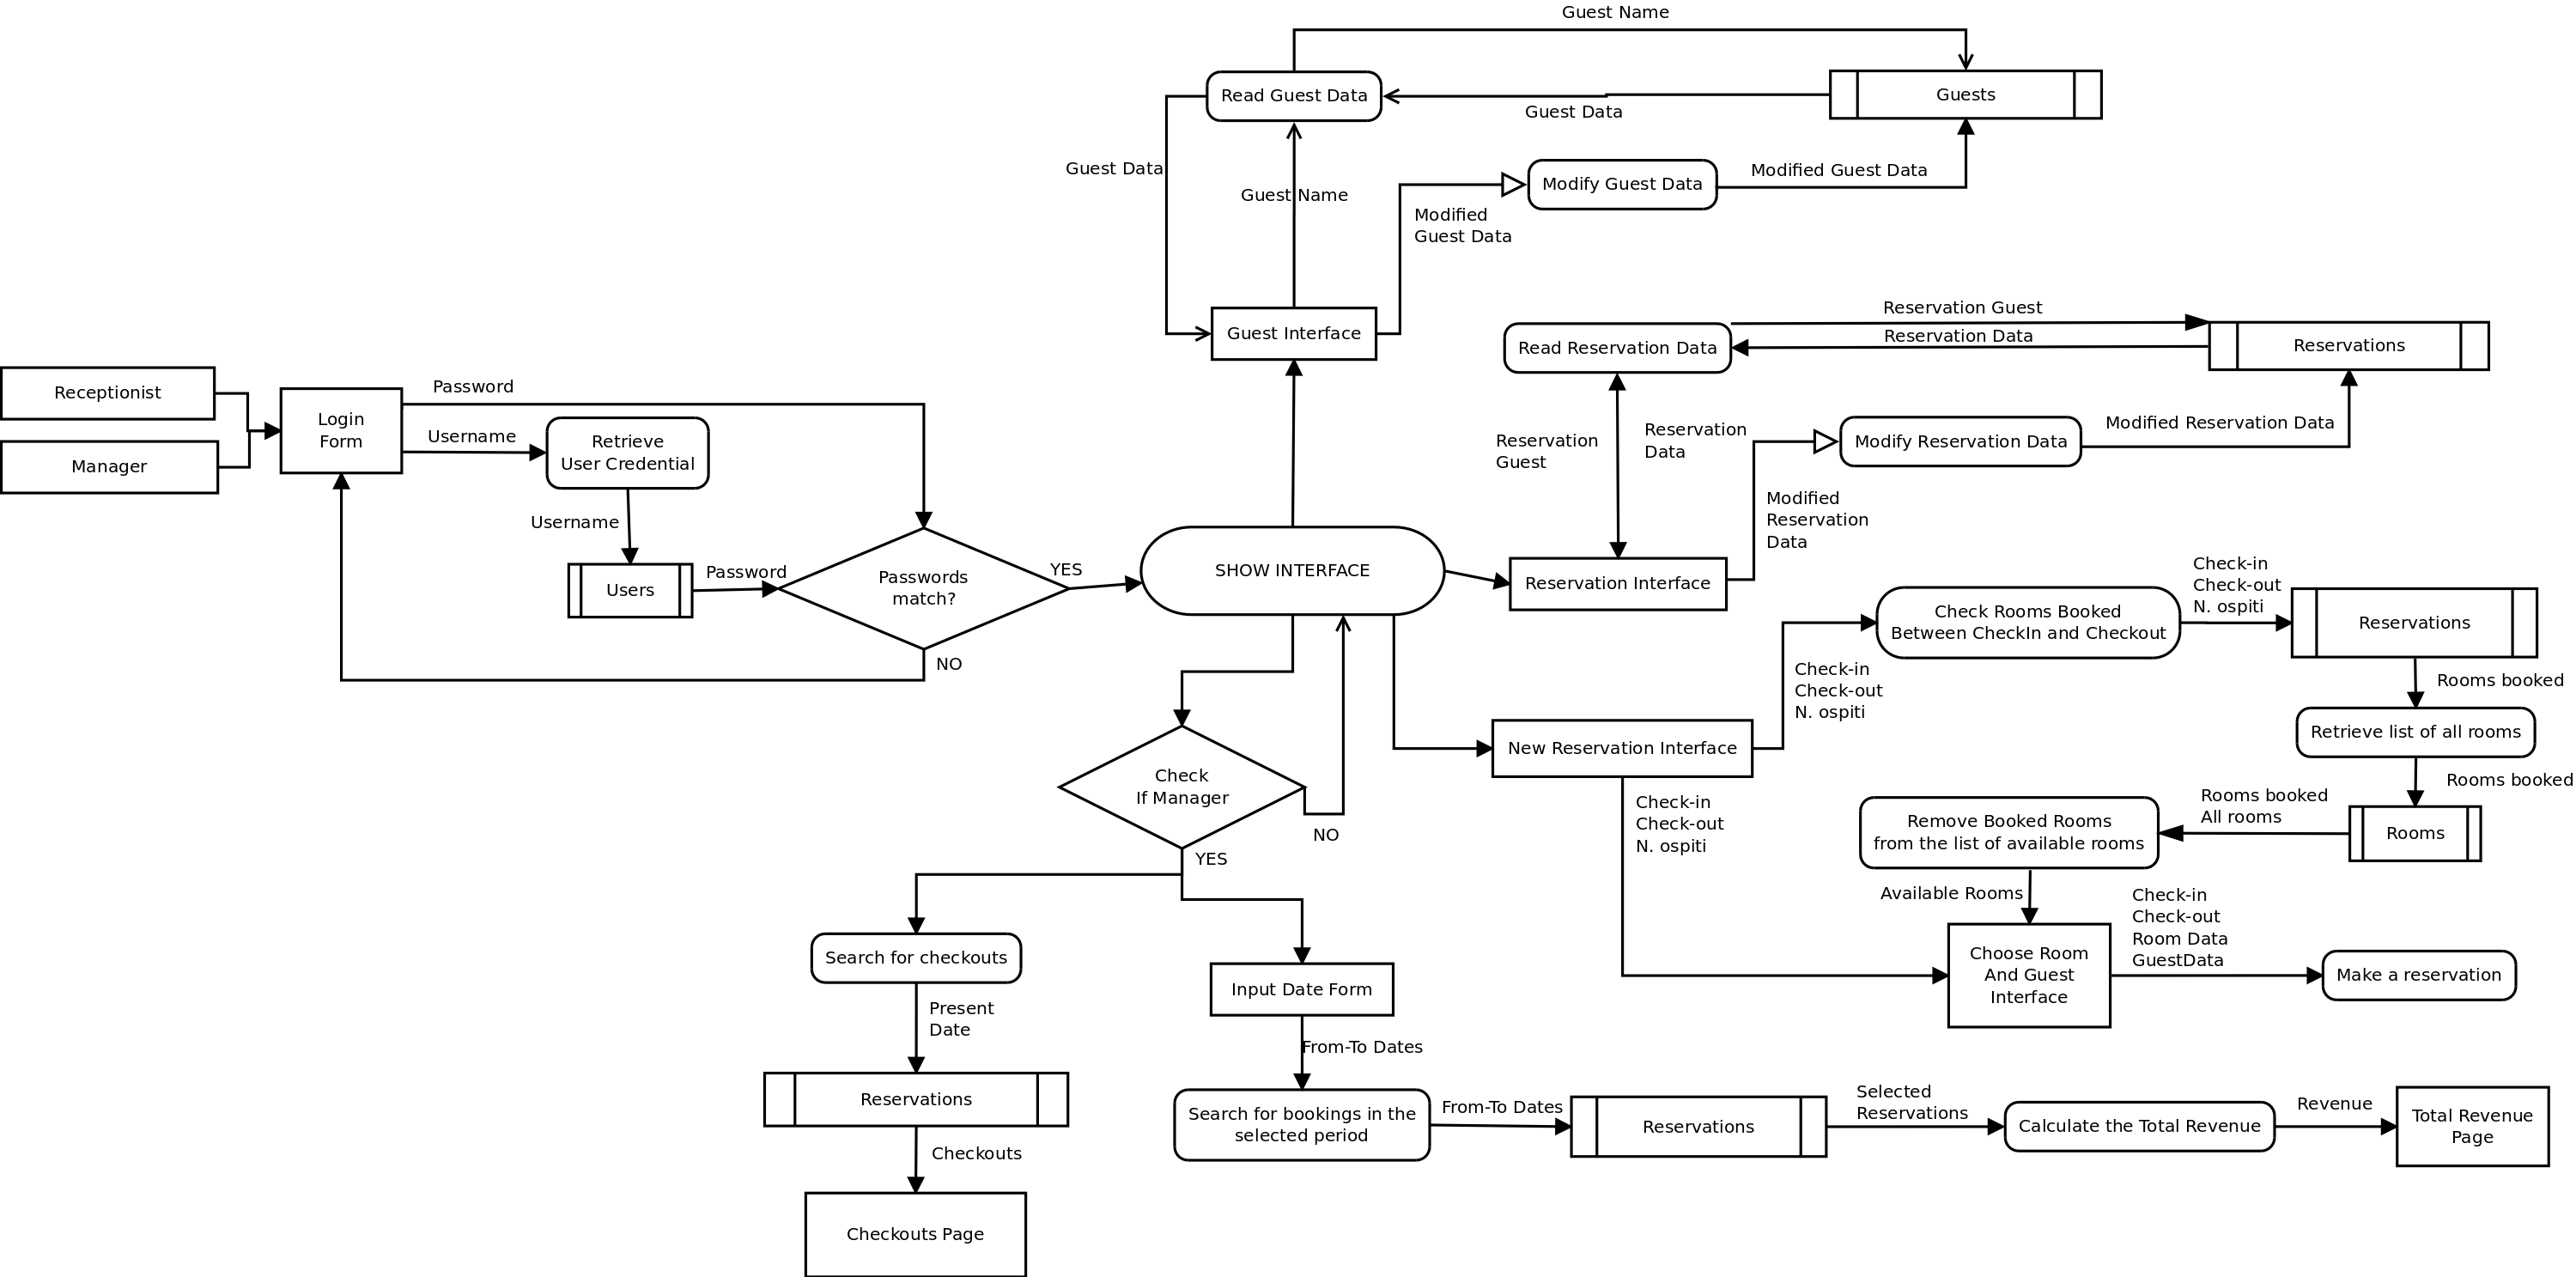
\includepdf[angle=90]{Diagram3}

\subsection{Elementary Process}

\begin{description}
  
    \item[Login Form:] \hfill \\
      A form to login in the system interface
    \item[Retrive User Credential:] \hfill \\
      Retrive the user credential for the users database table
    \item[Users (database):] \hfill \\
      Where the user credential and information are stored
    \item[Password Match?:] \hfill \\
      Check if the user credential input match with the data in users database table

    \item[Guest Interface:] \hfill \\
      a page where the guest information are managed
    \item[Read Guest Data:] \hfill \\
      read all the information about the guest from the database
    \item[Modify Guest Data:] \hfill \\
      a function to modify all or a part of the information about a guest
    \item[Guest (database):] \hfill \\
      where all guest informations are stored

    \item[Reservation Interface:] \hfill \\
      a page where the reservation information are managed
    \item[Read Reservation Data:] \hfill \\
      read all the reservation’s data of a guest from the database
    \item[Modify Reservation Data:] \hfill \\
      a function to modify the reservation data
    \item[Reservations (database):] \hfill \\
      where all the reservations are stored

    \item[New Reservation Interface:] \hfill \\
      a page where the user can do a new reservation
    \item[Retrive List Of All Rooms:] \hfill \\
      get the list of all the hotel rooms
    \item[Remove Booked Rooms From The List of Available Rooms:] \hfill \\
      remove the booked rooms in the selected period from the list of the hotel’s rooms
    \item[Choose Room And Guest interface:] \hfill \\
      a page where the user can choose the room and input the guest information
    \item[Make A Reservation:] \hfill \\
      the reservation is done and stored in the database

    \item[Check If Manager:] \hfill \\
      check if the user is logged as manager
    \item[Search for Check-OUTs:] \hfill \\
      search all the check-out of today or a specific day
    \item[Check-OUTs Page:] \hfill \\
      a page where manager can see all the check-out
    \item[Input Date Form:] \hfill \\
      a form  where input the date for the begin/end of a period
    \item[Search For Bookings In The Selected Period:] \hfill \\
      Search for all the booking made in the selected pariod
    \item[Calculate The Total Revenue:] \hfill \\
      Sum all the revenue from the booking of the period
    \item[Total Revenue Page:] \hfill \\
      show the total revenue in the selected period

\end{description}

\subsection{Data Structures}
  
\begin{description}
    
  \item[username:] \hfill \\ The indentifier used by the manager or receptionists to login 
    
  \item[password:] \hfill \\ The secret word used to verify the user's identity
    
  \item[Guest Name:] \hfill \\ Name of a guest searched in the database
    
  \item[Guest Data:] \hfill \\ All the information of a guest founded in the database
    
  \item[Modified Guest Data:] \hfill \\ Information modified by the user updating the guests data in the database

  \item[Reservation Guest:] \hfill \\ The name of the guest 
    
  \item[Reservation Data:] \hfill \\ All the information of a reservation founded in the database
    
  \item[Modified Reservation data:] \hfill \\ Information modified by the user updating the reservation data in the database

  \item[Check In/ Check Out:] \hfill \\ The data of arriving and departuring of a guest used to check the avaliability of the rooms in that period
    
  \item[Rooms booked:] \hfill \\ all the rooms not available for the indicated period
    
  \item[Available rooms:] \hfill \\ All the rooms available for the indicated period
    
  \item[All room:] \hfill \\ The list of all the room in the Hotel
    
  \item[Room Data:] \hfill \\ All the information of a room founded in the database
    
  \item[Checkouts:] \hfill \\ The reservation founded that end today
    
  \item[From/to dates:] \hfill \\ a period selected by the manager to show the reveneues in that period
    
\end {description}
